\documentclass[UTF8,zihao=-4]{ctexart}
\usepackage[a4paper,margin=2.5cm]{geometry}
\usepackage{amsmath, amssymb, amsthm}
\usepackage{bm}
\usepackage{hyperref}
\usepackage{graphicx}
\usepackage{caption}
\usepackage{listings}
\usepackage{xcolor}
\usepackage{float}
\usepackage{booktabs}
\usepackage{longtable}
\usepackage{multirow}
\usepackage{placeins}
\graphicspath{{figures/}}

% 代码样式
\lstdefinestyle{code}{
  basicstyle=\ttfamily\small,
  numbers=left,
  numberstyle=\tiny,
  numbersep=8pt,
  keywordstyle=\color{blue},
  commentstyle=\color{teal!70!black},
  stringstyle=\color{orange!70!black},
  showstringspaces=false,
  breaklines=true,
  frame=single,
  framerule=0.3pt,
  rulecolor=\color{black!15}
}
\lstset{style=code}

\title{高效推理实战:逐 token 生成、推测解码、量化与推理引擎}
\author{}
\date{\today}

\begin{document}
\maketitle

\section{推理流程(Token-by-Token Generation)}
\subsection{自回归流水线概述}
大语言模型(LLM)在推理阶段遵循自回归生成范式:模型逐步读取历史 token 序列 $x_{<t}$,在输出分布中采样下一个 token $x_t$。这一过程由嵌入层、注意力层、前馈网络、归一化层和输出投影组成,并借助 KV Cache(键值缓存)避免对历史 token 进行重复计算。图\ref{fig:token_pipeline} 展示了标准的逐 token 生成流水线。
\begin{figure}[H]
  \centering
  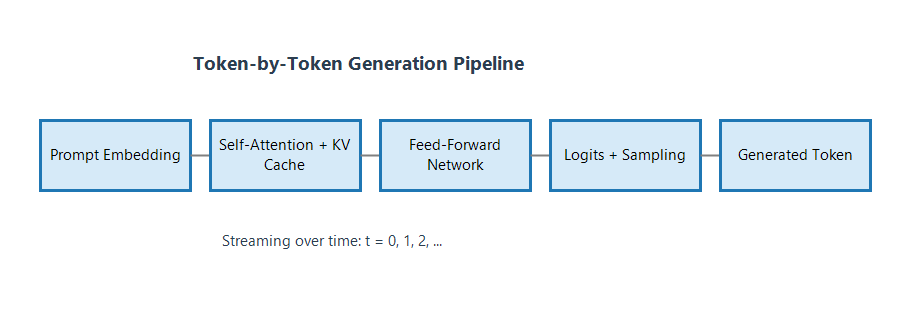
\includegraphics[width=0.85\textwidth]{token_generation_pipeline.png}
  \caption{逐 token 生成流水线:每一步均复用历史状态,避免全序列重复前向。}
  \label{fig:token_pipeline}
\end{figure}
关键特性总结如下:
\begin{itemize}
  \item \textbf{线性延迟累加:} 每生成一个 token 都需要完整的前向传播,因此单次响应时延与生成长度成正比。
  \item \textbf{复用历史状态:} KV Cache 存储历史层的键和值向量,将注意力计算复杂度从 $O(n^2)$ 降为 $O(n)$。
  \item \textbf{解耦采样策略:} 采样策略(Top-$k$、Top-$p$、温度等)在 logits 输出后执行,便于根据业务需求调整多样性与稳定性。
\end{itemize}

\subsection{批处理与流水并行}
在线服务往往通过批处理(batching)与流水线并行(pipelining)提高吞吐。常见策略包括:
\begin{itemize}
  \item \textbf{静态批:} 对同一批请求在 prompt 阶段进行并行前向,有效利用 GPU 张量核心。
  \item \textbf{动态批:} 通过请求调度器实时将多个生成中的会话合并,保持 GPU 利用率。需要在每步生成后切分结果,避免响应交错。
  \item \textbf{流水线并行:} 将模型分段部署在多块 GPU 上,输入 token 在流水线中逐层传递,减少单卡显存与推理时间。
\end{itemize}
调度器需要解决\textbf{批内不均衡}问题:不同会话生成长度差异导致部分请求提前完成,进而降低有效利用率。常用方法包括:
\begin{enumerate}
  \item 缩短最大生成长度或对长文本请求使用分段召回策略;
  \item 对正在生成的请求进行优先级排序,优先处理临界时延任务;
  \item 将批量拆分为“暖批”(prompt 阶段)和“热批”(token 阶段)两类,分别优化调度算法。
\end{enumerate}

\subsection{延迟优化与可见性}
要实现在业务 SLA(服务等级协议)下的稳定响应,需要从以下维度优化延迟:
\begin{itemize}
  \item \textbf{模型层面:} 合并 LayerNorm、残差和 MLP kernel,使用 FlashAttention/Fused MLP 减少内存访问;启用张量并行缩短单步计算时间。
  \item \textbf{运行时层面:} 使用多线程异步 IO、固定内存池减少频繁申请,记录每一步的 GPU kernel 时延用于瓶颈诊断。
  \item \textbf{系统层面:} 减少网络复制(如 Serverless 场景中的跨机数据传输)、采用零拷贝序列化协议、在推理节点旁路部署缓存层。
\end{itemize}
可观测性工具(如 NVIDIA Nsight、PyTorch Profiler)可用于定位 kernel 排队、拷贝开销、调度阻塞等问题。结合 SLA 控制图实时监控响应延迟的分位数(P50/P95/P99),及时调整批大小和优先级策略。

\section{Speculative Decoding 与 KV Cache 复用}
\subsection{算法原理}
Speculative Decoding 通过“主模型 + 草稿模型”协同生成候选 token,以减少主模型推理次数。核心流程如下:
\begin{enumerate}
  \item 选择一个轻量草稿模型(Draft Model),在相同上下文下生成若干候选序列 $\hat{x}_{t:t+k}$。
  \item 将候选序列逐 token 送入主模型(Target Model),验证每个 token 的概率是否满足接受条件(通常基于拒绝采样)。
  \item 当主模型接受候选 token 时,直接复用草稿模型推理出的 KV 状态,加速后续解码;若拒绝,则回退到主模型逐 token 推理。
\end{enumerate}
图\ref{fig:speculative} 展示了一个典型的验证流程:草稿模型一次性提出多个候选,主模型对每个候选进行快速校验与对齐。
\begin{figure}[H]
  \centering
  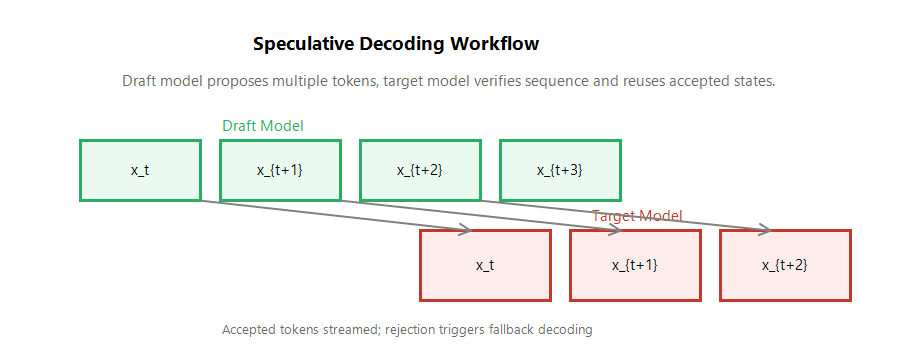
\includegraphics[width=0.85\textwidth]{speculative_decoding.png}
  \caption{Speculative Decoding:草稿模型并行生成候选,主模型验证并复用已接受的 KV 状态。}
  \label{fig:speculative}
\end{figure}

\subsection{接受准则与分布对齐}
为了保证生成质量,主模型需验证候选 token 的条件概率。设主模型分布为 $p_\theta$,草稿模型分布为 $q_\phi$,则对候选 token $x$ 的接受概率为:
\begin{equation}
  \alpha(x) = \min\left(1, \frac{p_\theta(x \mid x_{<t})}{q_\phi(x \mid x_{<t})}\right).
\end{equation}
若 $\alpha(x) < 1$ 则以概率 $\alpha(x)$ 接受,否则拒绝并重新从主模型采样。实践中,为避免频繁拒绝:
\begin{itemize}
  \item 通过蒸馏或连续微调,将草稿模型训练到与主模型接近的分布;
  \item 对草稿模型的 logits 施加温度缩放,鼓励其输出更保守的高置信度 token;
  \item 调整草稿模型输出长度 $k$,在吞吐与拒绝率之间寻找平衡。
\end{itemize}

\subsection{KV Cache 复用策略}
Speculative Decoding 的额外收益在于避免重复计算 KV Cache。实现要点包括:
\begin{itemize}
  \item \textbf{共享缓存格式:} 草稿模型与主模型需使用一致的张量布局(hidden size、头数、precision)。若主模型更大,可将草稿模型的 KV 张量嵌入主模型缓存。
  \item \textbf{懒惰更新:} 当主模型接受草稿 token 时,仅标记相应 KV 块为“已验证”;拒绝时延迟写入,避免在 GPU 上发生昂贵的回滚。
  \item \textbf{多会话调度:} 对批量请求,可在验证阶段对不同会话采用错位调度,最大化主模型的并行度。
\end{itemize}
在大部分公开实验中,Speculative Decoding 可带来 $1.5\text{--}2.5\times$ 的吞吐提升,尤其适用于主模型较大、草稿模型可放在同一 GPU 的场景。

\subsection{边界情况与工程实践}
\begin{itemize}
  \item \textbf{长上下文:} 草稿模型在超长上下文上可能积累误差,可定期强制同步至主模型 token,防止分布漂移。
  \item \textbf{多样性生成:} 当启用高温度或 nucleus sampling 时,草稿模型更易提出主模型拒绝的 token,需要动态调整候选长度。
  \item \textbf{故障回退:} 若草稿模型失效(如显存不足),运行时应自动降级为常规解码以保障可用性。
\end{itemize}

\section{模型量化(4bit, 8bit, GPTQ, AWQ)}
\subsection{基础概念与性能权衡}
量化通过降低权重与激活的数据精度(如 FP16 $\rightarrow$ INT8/INT4),显著减少模型显存与带宽需求。设权重向量为 $w \in \mathbb{R}^n$,量化操作可表示为:
\begin{equation}
  \tilde{w} = s \cdot \text{clip}\left(\text{round}\left(\frac{w}{s}\right), q_{\min}, q_{\max}\right),
\end{equation}
其中 $s$ 为缩放因子,$q_{\min}, q_{\max}$ 由量化位宽决定。主要权衡包括:
\begin{itemize}
  \item \textbf{精度损失:} 位宽越低,量化误差越大;需通过校准或感知训练补偿。
  \item \textbf{吞吐提升:} 低位宽减少内存访问,提升 GPU/CPU 算力利用率。
  \item \textbf{部署复杂度:} 需提供定制 kernel 支持混合精度计算与快速 dequant。
\end{itemize}

\subsection{8bit 量化(如 LLM.int8)}
8bit 量化通常对激活采用逐通道缩放,对权重采用逐列或逐矩阵缩放,以保证矩阵乘法精度。典型方案:
\begin{itemize}
  \item \textbf{LLM.int8:} 在矩阵乘法中将高方差行拆分为 FP16 计算,其余部分使用 INT8,实现接近无损的推理质量。
  \item \textbf{SmoothQuant:} 对权重和激活进行共同缩放,缓解激活分布的长尾问题,适用于在线服务的端到端 INT8 部署。
\end{itemize}
优点在于实现简单、精度损失极小,但显存压缩比例有限(约 $2\times$)。

\subsection{4bit 量化与 GPTQ}
4bit 量化可将权重存储压缩至原始 FP16 的 1/4。GPTQ(Gradient Post-Training Quantization)通过二阶近似在每层选择最优量化权重:
\begin{enumerate}
  \item 对每一层收集校准数据,计算 Hessian 对角近似(梯度平方期望)。
  \item 逐列拟合量化误差,选择最小化损失的量化值;残差通过回代传播到剩余权重。
  \item 支持混合精度:对敏感列保留更高位宽,提高整体准确率。
\end{enumerate}
GPTQ 可在无梯度的情况下完成量化,适合已有训练模型的离线压缩。缺点是需要较大的校准批量,且不含激活量化。

\subsection{AWQ 与激活感知量化}
AWQ(Activation-aware Weight Quantization)针对注意力与 MLP 层的激活分布进行校准,通过选择“关键通道”保持更高精度。其核心思想是:
\begin{itemize}
  \item 统计激活对输出的敏感度,将重要通道划分为高保真集合;
  \item 对关键通道保留更大的缩放因子(甚至更高位宽),非关键通道使用标准 INT4;
  \item 提供推理阶段的自适应缩放,使模型在不同输入分布下保持稳定。
\end{itemize}
AWQ 在不增加显存的前提下将困惑度降至接近 FP16 水平,已与多种推理引擎(如 TensorRT-LLM、vLLM)集成。

\subsection{量化策略对比}
\begin{longtable}{p{3cm}p{3cm}p{4cm}p{4cm}}
\toprule
方案 & 位宽 & 主要特点 & 适用场景 \\
\midrule
LLM.int8 / SmoothQuant & 8bit & 精度损失小,激活逐通道缩放 & 云端在线服务,模型较大但对精度要求高 \\
GPTQ & 4bit & 后训练量化,逐列二阶拟合 & 离线部署、边缘设备,兼顾压缩比与精度 \\
AWQ & 4bit & 激活感知,关键通道保留高精度 & 超长上下文、对注意力敏感的任务 \\
QLoRA & 4bit 权重 + 16bit 低秩适配器 & 量化基础模型,保持微调灵活性 & 参数高效微调,降低显存成本 \\
\bottomrule
\end{longtable}
实际部署中常见组合是“权重量化 + 激活半精度”,并针对注意力与输出层保留更高精度以控制误差。推理引擎需提供张量核或自定义 kernel 以减少 dequant/quant 的额外时间。

\section{高效推理框架(vLLM, TGI, Exllama)}
\subsection{vLLM:PagedAttention 与连续批处理}
vLLM 将显存视为分页内存,提出 PagedAttention 技术,将 KV Cache 按页管理,实现以下优势:
\begin{itemize}
  \item \textbf{零碎片化:} 通过页表映射解决多会话 KV 分配不均的问题,大幅提升显存利用率。
  \item \textbf{连续批处理(Continuous Batching):} 动态插入新请求到正在执行的批次中,提高吞吐同时保持稳定延迟。
  \item \textbf{统一接口:} 提供 OpenAI 相同 API 语义,兼容多种模型权重格式(HuggingFace、ggml、TensorRT-LLM 转换)。
\end{itemize}
vLLM 也支持 Speculative Decoding、Prefix Caching 等高级功能,适合作为多租户推理服务的基础层。

\subsection{Text Generation Inference (TGI)}
TGI 是 HuggingFace 发布的生产级推理服务,重点在于端到端部署体验:
\begin{itemize}
  \item \textbf{高性能内核:} 内置 FlashAttention、PagedAttention、Fused MLP 等优化 kernel,并可与 BetterTransformer 集成。
  \item \textbf{服务编排:} 支持分布式张量并行、模型切片加载、请求路由、负载均衡、token 限额控制等生产特性。
  \item \textbf{易于运维:} 基于 Rust + Python 实现,提供 Prometheus 监控、日志聚合、热更新等能力,适用于大规模 API 服务。
\end{itemize}
在部署流程上,TGI 可直接接入 HuggingFace Hub 模型仓库,通过 YAML 配置启用量化、LoRA 合并、LoRA 动态加载等能力。

\subsection{Exllama:轻量级本地推理}
Exllama 针对 4bit 量化模型进行了高度优化,特别适合消费级 GPU 和边缘设备:
\begin{itemize}
  \item \textbf{专用内核:} 针对 GPTQ 权重格式实现高效的稀疏矩阵乘法和自定义缓存布局,显著提高 4bit 推理速度。
  \item \textbf{显存友好:} 将 KV Cache 与权重分离存储,支持大语言模型在 12GB 甚至更低显存的 GPU 上运行。
  \item \textbf{易于集成:} 提供 Python 接口与文本生成前端,广泛用于本地部署、离线辅助工具与实验研究。
\end{itemize}
尽管 Exllama 在分布式和服务化能力上不及 vLLM/TGI,但在本地化、隐私保护、快速迭代场景中具有独特优势。

\subsection{框架选择指南}
不同框架侧重点如下:
\begin{itemize}
  \item 若追求\textbf{最高吞吐与多租户调度},选择 vLLM;
  \item 若关注\textbf{生产级部署与监控治理},选择 TGI;
  \item 若需要\textbf{轻量本地推理或 4bit 优化},选择 Exllama;
  \item 在 GPU 资源有限时,可结合量化与 Speculative Decoding,将 Exllama 作为草稿模型,vLLM 提供主模型服务。
\end{itemize}

\section*{实践建议}
\begin{itemize}
  \item 将推理流程拆分为 prompt 预处理、逐步生成、后处理三个阶段,分别度量延迟与显存占用。
  \item 对 Speculative Decoding、量化等优化项采用 A/B 测试验证效果,记录吞吐、拒绝率、模型评分等指标。
  \item 结合推理框架提供的调度 API,对业务负载进行高峰/低谷评估,并预留缓冲资源应对突发流量。
\end{itemize}

\section*{参考文献}
\begin{itemize}
  \item Leviathan et al. ``Fast Inference from Transformers via Speculative Decoding.'' ICML, 2023.
  \item Frantar et al. ``GPTQ: Accurate Post-Training Quantization for Generative Pre-trained Transformers.'' NeurIPS, 2022.
  \item Lin et al. ``AWQ: Activation-aware Weight Quantization for LLM Compression and Acceleration.'' arXiv, 2023.
  \item Kwon et al. ``Efficient Memory Management for Large Language Model Serving with PagedAttention.'' arXiv, 2023.
  \item HuggingFace. ``Text Generation Inference: Scalable Production-ready LLM Serving.'' Technical Report, 2024.
\end{itemize}

\end{document}

